\icode{E-MI-MU-L2-261106-001}
（多选）
如图所示，固定的半球面右侧是光滑的，左侧是粗糙的，\(O\)点为球心，\(A\)、\(B\)为两个完全相同的小物块（可视为质点），小物块\(A\)静止在球面的左侧，受到的摩擦力大小为\(F_1\)，对	球面的压力大小为\(N_1\)；小物块\(B\)在水平力\(F_2\)作用下静止在球面的右侧，对球面的压力大小为\(N_2\)，已知两小物块与球心连线和竖直方向的夹角均为\(\theta\)，则\paren[]

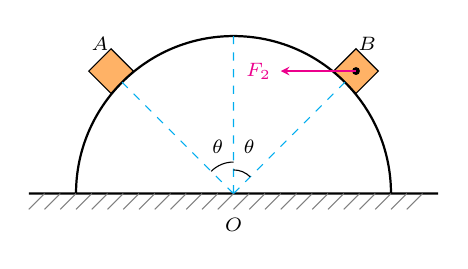
\begin{tikzpicture}[>=stealth,font=\scriptsize]
	\draw[fill=orange!60,rotate=45] (-.2,2) rectangle(.2,2.4);
	\draw[fill=orange!60,rotate=-45] (-.2,2) rectangle(.2,2.4);
	\draw[thick] (2,0) arc(0:180:2) (-2.6,0)--(2.6,0);
	\draw[dashed,cyan] (0,0)--(45:2) (0,0)--(135:2) (0,0)--(0,2);
	\draw (45:.3) arc(45:90:.3) (0,.4) arc(90:135:.4);
	\coordinate (O) at({1.1*sqrt(2)},{1.1*sqrt(2)});
	\fill (O) circle(.05);
	\draw[->,magenta] (O)--(O-|.6,.2)node[left]{\(F_2\)};
	\foreach \x in {-2.6,-2.4,...,2.4}
		\draw[gray] (\x,-.2)--++(.2,.2);
	\node at(45:2.4)[above]{\(B\)};
	\node at(135:2.4)[above]{\(A\)};
	\node at(-.2,.6){\(\theta\)};
	\node at(.2,.6){\(\theta\)};
	\node at(0,-.4){\(O\)};
\end{tikzpicture}
\begin{choices}
	\item\(F_1:F_2 = \cos\theta:1\)
	\item\(F_1:F_2 = \sin\theta:1\)
	\item\(N_1:N_2 = \cos^2\theta:1\)
	\item\(N_1:N_2 = \sin^2\theta:1\)
\end{choices}
\begin{answer}
	AC\qquad 提示：
\end{answer}